%%
%% Author: nikolas
%% 11.03.18
%%

% Preamble
\documentclass[11pt]{article}

% Packages
%\usepackage{a4wide}
\usepackage[a4paper, margin=2.22cm]{geometry}
\usepackage[german]{babel}
\usepackage[utf8]{inputenc}
\usepackage{amsmath}
\usepackage{amssymb}
\usepackage{amsthm}
\usepackage{mathtools}
\usepackage{enumitem}
\usepackage[plain]{algorithm}
\usepackage{algorithmic}
\usepackage{graphicx}
\usepackage[font=small]{caption}
%\usepackage{hyperref} % Makes citations clickable


\newcommand{\R}{\mathbb{R}}
\newcommand{\n}{\newline}
\renewcommand{\baselinestretch}{1.15} % line distance
\renewcommand{\proofname}{\Beweis} % name proofs 'Beweis'
\addto\captionsgerman{\renewcommand{\figurename}{Abb.}} % name figures 'Abb.' (change it for babel)

\setitemize{itemsep=0mm} % itemize line distance
\setenumerate{label=(\arabic*),itemsep=0mm} % enumerate labeling and line distance
\allowdisplaybreaks % make math equations breakable

\newtheorem{theorem}{Satz}[section]
\newtheorem{lemma}[theorem]{Lemma}
\newtheorem{definition}[theorem]{Definition}
\newtheorem{corollary}[theorem]{Korollar}

% Headline
\title{Distanzerhaltende Approximation von Kantenzügen}
\author{Nikolas Klug}
\date{Sommersemester 2018
	\\ Universität Augsburg
	\\ Seminar Algorithmen und Datenstrukturen
	}


% Document
\begin{document}
    \maketitle

    \begin{abstract}
        Diese Seminararbeit basiert auf \glqq Distance-preserving approximations of polygonal paths\grqq\ von J. Gudmundsson et al. (\cite{gudmundsson}). Sei $P = (p_1, p_2, \mathellipsis, p_n)$ ein Kantenzug und $t \geq 1$. Ein Kantenzug $Q$ approximiert $P$, falls er nur aus Punkten von $P$ besteht und falls die Längen seiner Kanten jeweils nur um einen Faktor $t$ von $P$ abweichen. Diese Arbeit stellt exakte und approximative Algorithmen dar, um $Q$ so zu berechnen, dass $Q$ entweder die minimale Zahl von Knoten besitzt oder für eine feste Knotenzahl 
        minimales $t$ hat.
    \end{abstract}

    \section{Einführung und Definitionen}
    \label{sec:intro}
		Ein \emph{(polygonaler) Kantenzug} $P = (p_1, p_2, \mathellipsis, p_n)$ ist eine Aneinanderreihung von Geradensegmenten, die für $1 \leq i < n$ jeweils $p_i$ und $p_{i+1}$ verbinden. 
	Bei den $p_i$ handelt es sich dabei um Punkte aus $\R^d$ (für $d \in \mathbb{N}$). Aufgrund der starken Ähnlichkeit zu Pfaden in (gerichteten) Graphen werden wir für Kantenzüge auch häufig Begriffe aus der Graphentheorie verwenden. 
	Beispielsweise heißen die Punkte des Kantenzuges auch Knoten, die verbindenden Geraden auch (gerichtete) Kanten etc.
	In anderen Vorlesungen und Fachbüchern werden und wurden die Begriffe Kantenzug und Pfad teilweise synonym verwendet, wir wollen diese hier aber - der besseren Verständlichkeit wegen -  klar unterscheiden.

    In der Realität kann ein solcher Kantenzug mitunter eine hohe Zahl von Knoten besitzen, von denen die meisten für die Anwendung uninteressant sind. 
    Hier ist es vorteilhaft, diesen Kantenzug durch einen ähnlichen Kantenzug mit deutlich weniger Kanten (und somit auch Knoten) zu approximieren, wobei sich wichtige Parameter allerdings nicht stark ändern. 
    In der Fachliteratur werden dabei zahlreiche verschiedene Parameter aufgeführt, die bei der Approximation erhalten werden sollen, einige davon sind die Fläche \cite{bose}, die der Pfad einschließt und die Distanz bzw. die Länge des Pfades \cite{gudmundsson}. 
    
    Ein Anwendungsszenario der Kantenzugapproximation liegt zum Beispiel bei der Erstellung und Vereinfachung von Karten. 
    Dort trifft man ständig auf polygonale Kantenzüge im \mbox{zwei-,} selten auch dreidimensionalen Raum: Straßen, Küstenlinien, Höhenlinien, Stadtumrisse und Landesgrenzen sind nur einige Beispiele. 
    Leider sind in den meisten Fällen nicht alle dieser Kantenzüge so einfach darzustellen wie beispielsweise die Grenze zwischen Libyen und Ägypten; betrachtet man die Weltkarte, fällt auf, dass die meisten Grenzen sogar sehr komplizierte Formen annehmen, die aus Tausenden, wenn nicht Zehntausenden, einzelnen Punkten bestehen.
    Möchte man nun eine Karte erstellen, ist klar, dass es im Allgemeinen nicht möglich und auch nicht wünschenswert ist, alle dieser Punkte darzustellen. 
    Genau an dieser Stelle liegt eine Anwendung der Kantenzugapproximation: Die Landesgrenze bzw. die anderen oben aufgeführten Beispiele werden durch einen Kantenzug approximiert, der aus deutlich weniger Punkten besteht, ohne dass sich ein wichtiger Parameter ändert, wie zum Beispiel die Länge.
    
    In dieser Arbeit soll es um Algorithmen gehen, die einen polygonalen Kantenzug unter ungefährer Einhaltung der Länge approximieren. 
    Dabei betrachten wir zunächst zwei exakte Algorithmen und später noch zwei approximative, die eine deutliche bessere Laufzeit aufweisen als die exakten. 
    
    Bevor wir uns den Algorithmen zuwenden, müssen wir jedoch einige Grundbegriffe definieren.
   
   \subsection{Definitionen}
   \label{subsec:def}
   
    Seien $u, v \in \R^d$. Wir definieren $|uv|$ als den euklidischen Abstand von $u$ und $v$.
    Ist $p_i, p_j \in P$, dann ist $\delta(p_i, p_j) \coloneqq \sum\limits_{k=i}^{j-1}{|p_k
    p_{k+1}|}$, also der euklidische Abstand dieser beiden Punkte entlang des Pfades $P$.
	\begin{lemma}
		\label{lem:triangle}
		Für alle Knoten $p_i, p_j \in P$ gilt $|p_ip_j| \leq \delta(p_i, p_j)$
	\end{lemma}
	\begin{proof}
		Die Strecke zwischen zwei Punkten in $\R^d$ ist immer die kürzeste Verbindung dieser beiden Punkte.
	\end{proof}
	Bis jetzt haben wir nur über distanzerhaltende Approximationen eines Kantenzugs geredet, ohne  festzulegen, was distanzerhaltend überhaupt bedeutet. Wir nennen eine Kante distanzerhaltend, wenn ihre Länge nur um einen bestimmten Faktor von der Länge des Pfade abweicht. Genauer:
	\begin{definition}[$t$-distanzerhaltend]
		\label{def:t-dist}
		Sind $p_i, p_j \in P$, dann ist die Kante $(p_i, p_j)$ genau dann \emph{$t$-distanzerhaltend}, wenn $\delta(p_i, p_j) \leq t \cdot |p_ip_j|$.
	\end{definition}
	
	Damit können wir jetzt definieren, was eine distanzerhaltende Approximation ist.

	\begin{definition}[$t$-distanzerhaltende Approximation]
		\label{def:t-distapp}
		Ein Kantenzug $Q = (p_{i_1}, p_{i_2}, \mathellipsis, p_{i_k})$ ist genau dann eine \emph{$t$-distanzerhaltende Approximation von $P = (p_1, p_2, \mathellipsis, p_n)$}, wenn beide der folgenden Bedingungen gelten.
		\begin{enumerate}
			\item $\displaystyle 1 = i_1 < i_2 < \mathellipsis < i_k = n$
			\item $\displaystyle \text{Für alle } 1 \leq l < k \text{ ist die Kante } (p_{i_l}, p_{i_{l+1}})$ des Kantenzugs $t$-distanzerhaltend
		\end{enumerate}
	\end{definition}
	
	Wir nennen eine t-distanzerhaltende Approximation eines Pfades \emph{minimal}, falls sie die geringst mögliche Zahl an Knoten besitzt.
	Der Quotient $\frac{\delta(p_i, p_j)}{|p_ip_j|}$ heißt \emph{Abweichung} vom Kantenzug.
	\begin{corollary}
		\label{cor:approximations}
		Sei $1 \leq t < t'$. Dann ist jede $t$-distanzerhaltende Approximation eines Pfades $P$ auch eine $t'$-distanzerhaltende Approximation von $P$.
	\end{corollary}

	In Zusammenhang mit der distanzerhaltenden Kantenzugapproximation stellen sich im Wesentlichen die folgenden zwei Probleme:
	
	\noindent Das \textbf{Minimum-Vertex-Path-Simplification Problem (MVPS)}: Liegt ein polygonaler Kantenzug $P$ und eine reelle Zahl $t \geq 1$ vor, soll eine kürzeste $t$-distanzerhaltende Approximation von $P$ berechnet werden.
	
	\noindent Das \textbf{Minimum-Dilation-Path-Simplification Problem (MDPS)}: Liegt ein polygonaler Kantenzug $P$ und eine natürliche Zahl $k$ vor, soll der kleinste Wert $t$ bestimmt werden, für den eine $t$-distanzerhaltende Approximation mit maximal $k$ Knoten existiert.

    \begin{figure}
    	\centering
    	\begin{minipage}{.8\linewidth}
    		 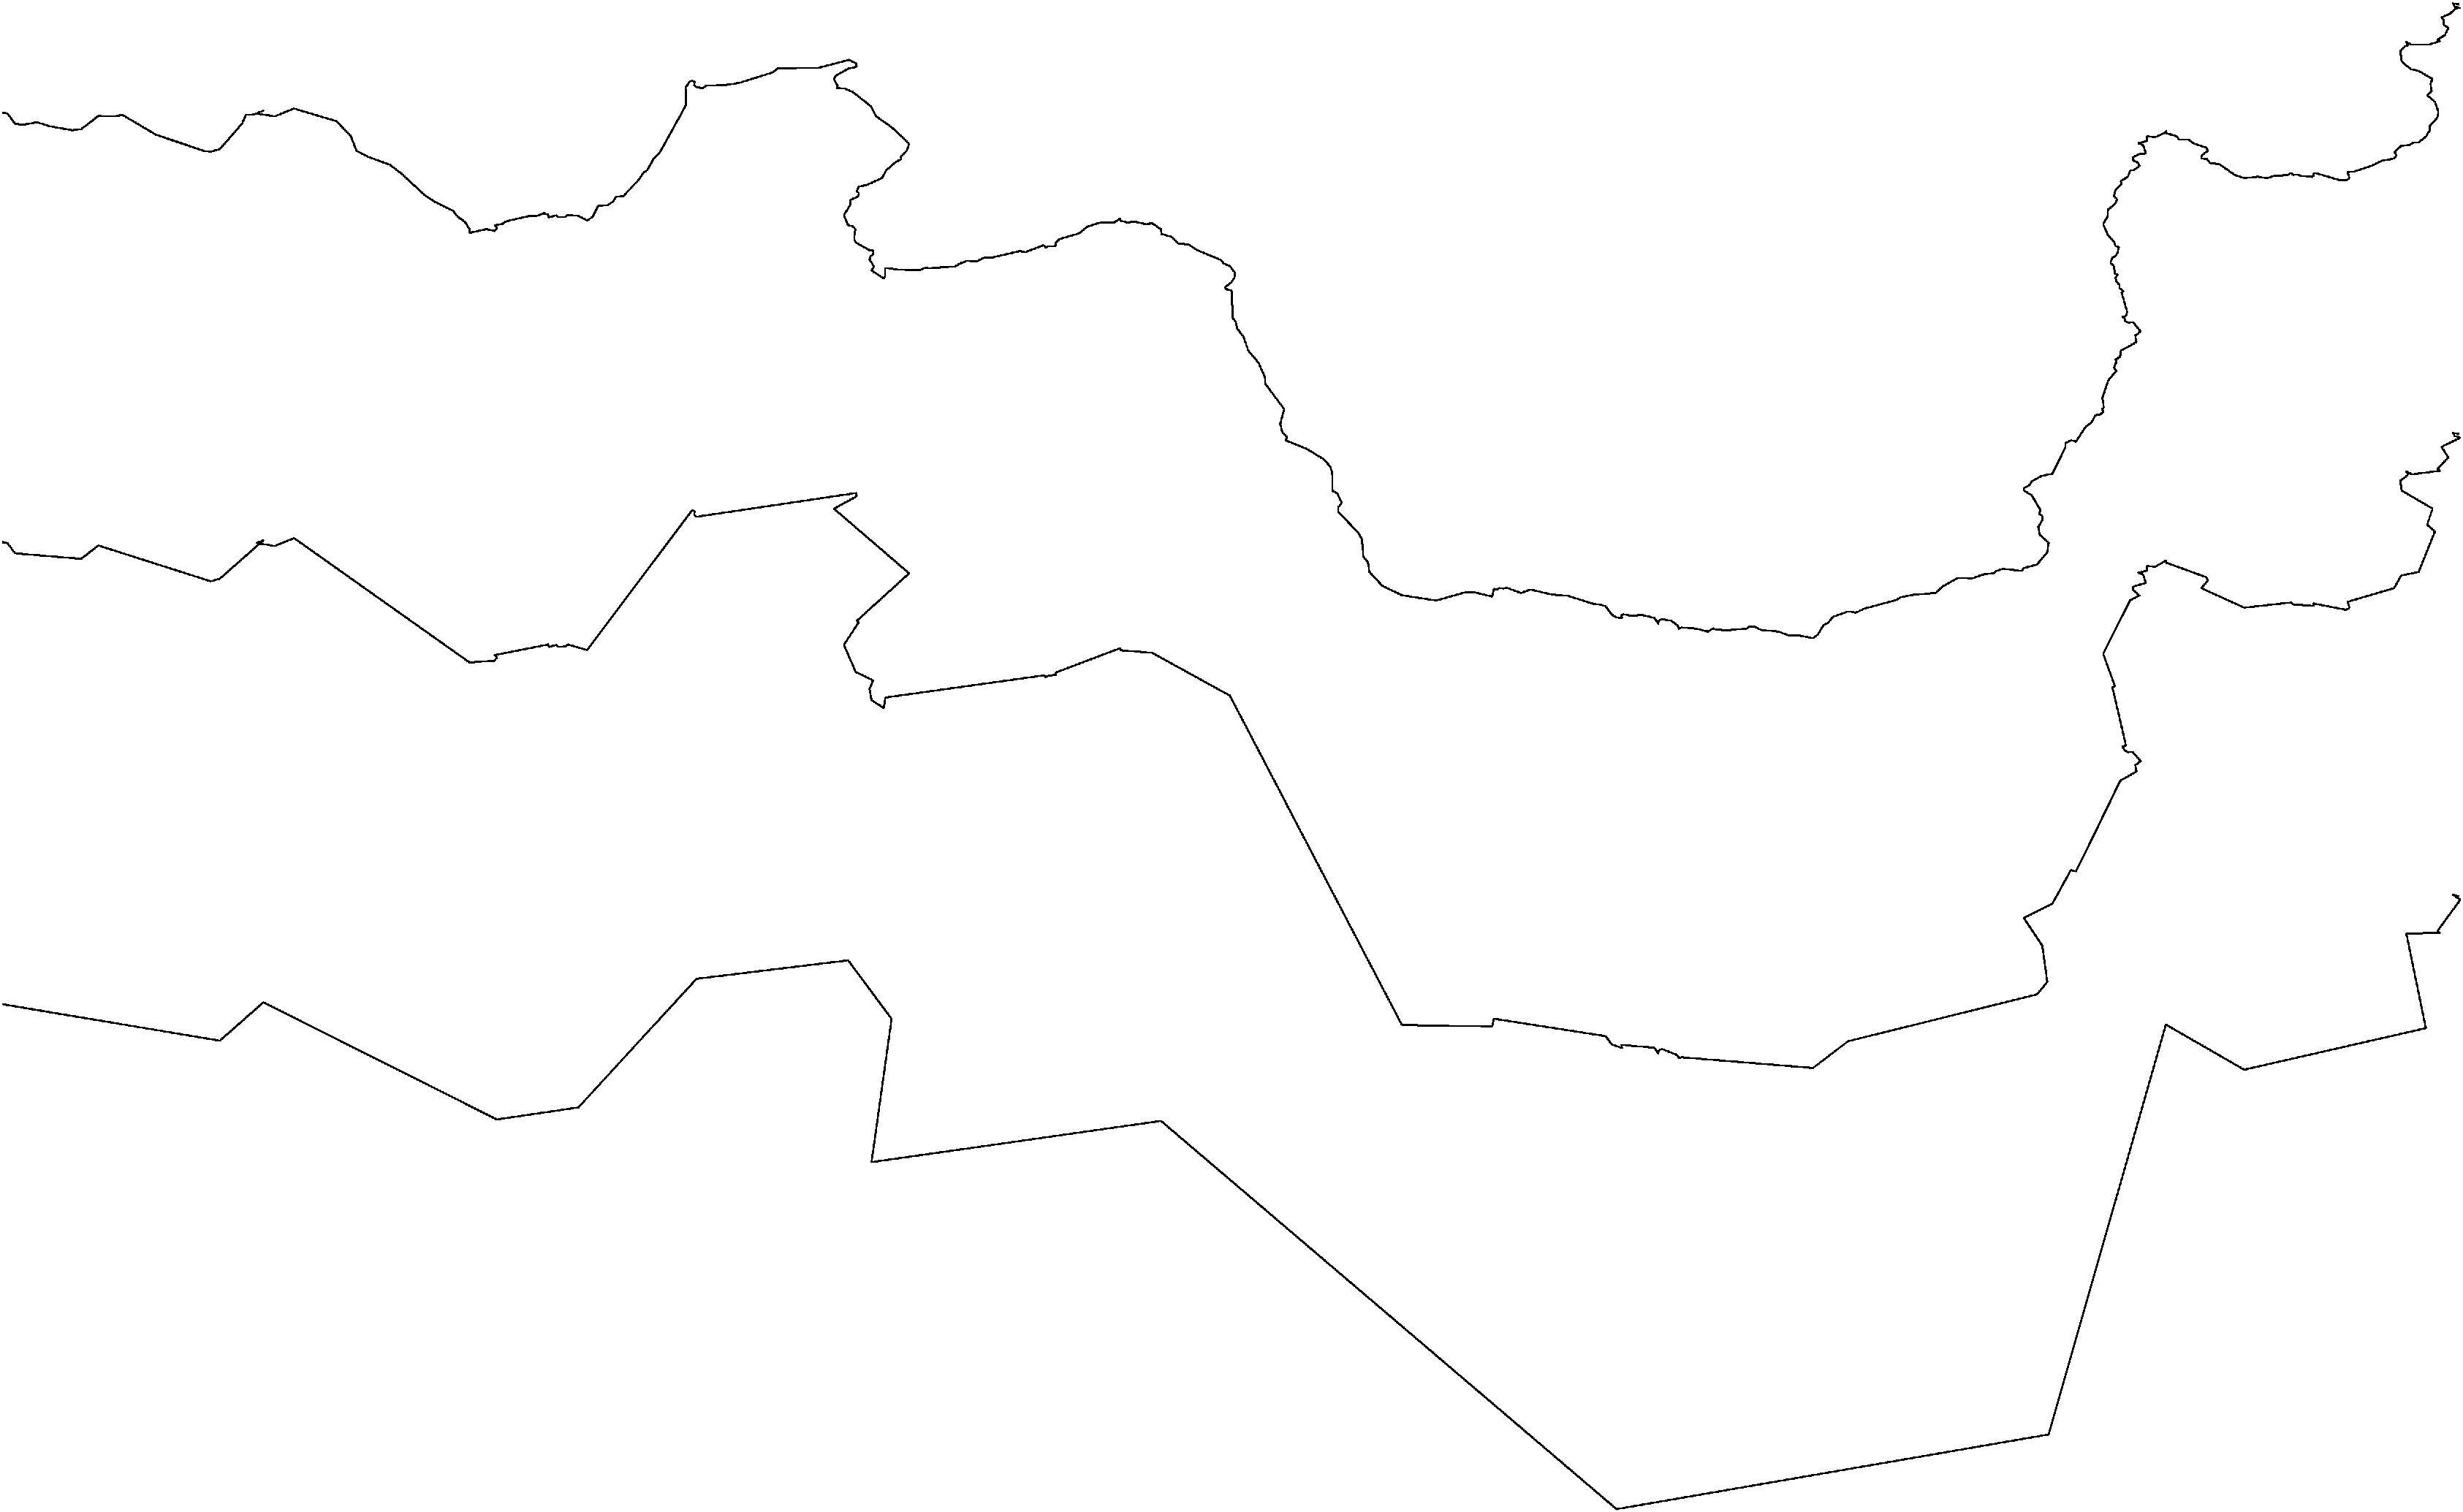
\includegraphics[scale=0.15]{approximation_example}
    	\end{minipage}
    	\caption{Kantenzug mit 430 Punkten (oben) und zwei Approximationen mit 126 bzw. 22 Punkten (mitte und unten), die aus dem approximativen Algorithmus für das MVPS-Problem mit jeweils $\epsilon = 0.05$ und $t = 1.05$ bzw. $t = 1.2$ berechnet wurden (Quelle: \cite{gudmundsson})}
    \end{figure}

    \section{Exakte Algorithmen für MVPS und MDPS}
    \label{sec:exact}
    	Zu Beginn betrachten wir zwei einfache exakte Algorithmen.
    Seien wieder $d\geq1$, $t>1$ und $P = (p_1, p_2, \mathellipsis, p_n)$ ein Kantenzug in $\R^d$. Sei weiter $P^*$ die Menge aller kürzesten $t$-distanzerhaltenden Approximationen
    
    Wir konstruieren jetzt den gerichteten Graphen $G_t = (V,E_t)$, wobei V genau aus den Knoten des Pfades $P$ besteht und 
    $E_t = \{(p_i, p_j) \in V\times V|\ i < j \text{ und } (p_i,p_j)\ \text{ist $t$-distanzerhaltend}\}$. $E_t$ ist also gerade die Menge aller $t$-distanzerhaltenden Kanten zwischen Knoten aus $V$. Zunächst beobachten wir, dass jede $t$-distanzerhaltende Approximation von $P$ einem Pfad in $G_t$ entspricht, da $G_t$ alle $t$-distanzerhaltenden Kanten zwischen Knoten von $P$ enthält. Andererseits ist auch jeder Pfad $Q = (p_{i_1}, p_{i_2}, \mathellipsis, p_{i_k})$ mit $1 = i_1 < i_2 < \mathellipsis < i_k = n$ in $G_t$ eine $t$-distanzerhaltende Approximation von $P$, da nur $t$-distanzerhaltende Kanten verwendet werden. Daraus folgt, dass auch $P^*$ in $G_t$ liegt. Jetzt müssen wir also nur noch ein Element aus $P^*$ ermitteln. Das ist leicht: Wir führen eine Breitensuche in $G_t$ mit Startknoten $p_1$ durch, bei der wir jeden Knoten mit der Nummer des Knotens beschriften, von dem aus er zum ersten Mal entdeckt wurde (also mit der Nummer seines Vaters im BFS-Baum). Am Ende lesen wir diese Beschriftung bei $p_n$ beginnend solange aus, bis wir $p_1$ erreichen. Der dadurch enstandene Pfad entpricht dann aufgrund der Eigenschaften der Breitensuche einem Kantenzug in $P^*$. 
    Nun betrachten wir noch die Laufzeit: Die Konstruktion von $G_t$ gelingt uns in $O(n^2)$, da wir für maximal $\binom{n}{2} = O(n^2)$ Kanten überprüfen müssen, ob diese $t$-distanzerhaltend sind. Sei $m$ die Zahl der Kanten in $G_t$, dann wissen wir aus  \cite{hagerup}, dass die Breitensuche $O(n+m)$ Zeit dauert. In unserem Fall ist $O(m) = O(n^2)$, und somit dauert die Breitensuche auch $O(n^2)$. Insbesondere haben wir:
    \begin{theorem}
    	\label{theo:mvpsex}
    	Das Minimum-Vertex-Path-Simplification Problem kann für Pfade mit n Knoten $O(n^2)$ gelöst werden.
    \end{theorem} 
    
    Als nächstes wollen wir uns überlegen, wie man das MDPS-Problem für eine feste Anzahl von Knoten $k$ lösen kann. Sei im Folgenden $\kappa_t$ die geringst mögliche Zahl von Knoten für eine $t$-distanzerhaltende Approximation von $P$.
	\begin{lemma}
		\label{lem:kappa}
		Sind $t, t' \in \R$ und $1 \leq t < t'$, dann ist $\kappa_t \geq \kappa_{t'}$.
	\end{lemma}
	\begin{proof}
		Wäre $\kappa_{t'} < \kappa_t$, hätte eine kürzeste $t'$-distanzerhaltende Approximation weniger Knoten als eine kürzeste $t$-distanzerhaltende. Aber jede $t$-distanzerhaltende Approximation von $P$ ist nach Lemma \ref{lem:approximations} auch eine $t'$-distanzerhaltende Approximation. Das ist ein Widerspruch. 
	\end{proof}
	
	Da $G_t$ maximal $O(n^2)$ Kanten enthält, gibt es eine endliche Zahl von $t$-Werten. Wir müssen also nur noch aus diesen Werten den geringsten Wert $t^*$ ermitteln, der gerade noch k Knoten oder weniger hat. Dazu definieren wir zunächst für $1\leq i < j \leq n$ $t^*_{ij} \coloneqq\frac{\delta(p_i, p_j)}{|p_i p_j|}$, also als die Abweichung der Kante $(p_i, p_j)$ vom Pfad. Sei nun $M\coloneqq\{t^*_{ij}\ |\ 1\leq i < j \leq n\}$. Wir wissen, dass $t^* \in M$, da die gesuchte Approximation eine Kante mit maximalen $t$-Wert hat, und $M$ gerade alle diese enthält. Wegen Lemma \ref{lem:kappa} wissen wir, das sich die $\kappa_t$ umgekehrt proportional zu den $t$-Werten verhalten. Sortieren wir jetzt $M$ zu $M'$, können wir in $M'$ nach $t^*$ suchen. Da $M$ $O(n^2)$ Elemente enthält, können wir $M$ nach \cite{hagerup} in $O(n^2\log n^2)=O(n^2\log n)$ sortieren. Für die Suche verwenden wir eine Binärsuche, bei der wir jeweils für den aktuell betrachteten $t$-Wert das MVPS lösen und dann abhängig vom Ergebnis entweder im rechten oder linken Teilbereich weitersuchen. 
	Eine gewöhnliche Binärsuche dauert bekanntermaßen $O(\log n)$ und mit Satz \ref{theo:mvpsex} ergibt sich auch hier eine Laufzeit von $O(n^2\log n)$. Wir halten fest:
	\begin{theorem}
		Das Minimum Dilation Path Simplification Problem kann für Pfade mit n Knoten in $O(n^2 \log n)$ gelöst werden.
	\end{theorem}
	
	Damit beschließen wir das Kapitel über exakte Algorithmen für das MVPS- und das MDPS-Problem und wenden uns approximativen Lösungen zu.

    
    \section{Approximative Algorithmen}
    \label{sec:approximative}
    
    Die beiden approximativen Algorithmen, die wir betrachten werden, basieren auf der sogenannten Zerlegung in wohl-separierte Paare. Dabei werden im weitesten Sinne die Punkte des Kantenzugs in verschiedenen Mengen zusammengefasst, die bestimmte Eigenschaften haben. Da diese Zerlegung einen wesentlichen Teil beider Algorithmen ausmacht, werden wir sie zunächst genauer definieren und einen Algorithmus zur Berechnung angeben.

    \subsection{Well-separated Pair Decomposition}
    \label{subsec:wspd}
    \begin{definition}[wohl-separiert]
   	\label{def:wellsep}
   	Seien $s > 0$ und $A$ und $B$ zwei endliche Mengen von Punkten in $\R^d$. 
   	$A$ und $B$ heißen \emph{wohl-separiert in Bezug zu $s$} (engl. well-separated), falls es zwei disjunkte Bälle $C_A$ und $C_B$ gibt, die denselben Radius $R$ haben, sodass $A \subseteq C_A$ und $B \subseteq C_B$ und die euklidische Distanz zwischen $C_A$ und $C_B$ mindestens $s\cdot R$ beträgt.

	$s$ ist dabei die \emph{Trennungsrate} der Mengen $A$ und $B$.
\end{definition}

Das folgende Lemma hält zwei wichtige Eigenschaften von zwei in Bezug zu $s$ wohl-separierten Mengen $A$ und $B$ fest.
\begin{lemma}
   	\label{lem:wellsep}
	Seien $a, a' \in A$ und $b, b' \in B$. Dann gilt:
	\begin{enumerate}
		\item $\displaystyle |aa'| \leq \frac{2}{s}\cdot|a'b'|$
		\item $\displaystyle |a'b'| \leq (1+\frac{4}{s})\cdot|ab|$
	\end{enumerate}
\end{lemma}
\begin{proof}
   	Zu 1. Ist $r$ der Radius von $C_A$ und $C_B$, so gilt $|aa'| \leq 2 \cdot r$. Da $A$ und $B$ wohl-separiert sind, gilt zudem $|a'b'| \geq s \cdot r$, was äquivalent ist zu $r \leq \frac{|a'b'|}{s}$. Durch Einsetzen folgt dann die Behauptung.
   	
   	Zu 2. Da $A$ und $B$ wohl-separiert in Bezug zu $s$ sind, und $C_A$ und $C_B$ beide denselben Radius $r$ haben, gilt $|a'b'| \leq s \cdot r + 4 \cdot r$. Ausklammern rechts ergibt $(1 + \frac{4}{s}) \cdot s \cdot r$. Da ja auch $s \cdot r \leq |ab|$, folgt durch Einsetzen die Behauptung.
\end{proof}

\begin{definition}[WSPD]
   	\label{def:wspd}
   	Sei $S \subseteq \R^d$ und $s > 0$. 
   	Eine Folge $\{A_i, B_i\}_{1 \leq i \leq m}$ von nicht-leeren Teilmengen von S ist genau dann eine \emph{Zerlegung in wohl-separierte Paare (engl. well-separated pair decomposition; WSPD)}, wenn gilt:
   	\begin{enumerate}[label={(\arabic*)}, itemsep=0mm]
   		\item $A_i \cap B_i = \emptyset$
   		\item Für alle $p, q \in S$ gibt es genau einen Index $1 \leq i \leq m$, sodass entweder $p \in A_i$ und $q \in B_i$ oder $q \in A_i$ und $p \in B_i$.
   		\item $A_i$ und $B_i$ sind wohl-separiert in Bezug zu $s$
   	\end{enumerate}
\end{definition}

\noindent $m$ nennen wir dabei die \emph{Größe} der WSPD.

Die WSPD bildet eine wichtige Grundlage für die beiden Algorithmen, die wir im Folgenden betrachten werden. 
Callahan und Kosaraju haben in \cite{callahan} gezeigt, dass man zu einer gegebenen Menge $L \subset \R^d$ der Größe $n$ eine WSPD  der Größe $m = O(s^dn)$ in $O(n\log n + s^dn)$ Zeit berechnen kann. 
Dabei wird zunächst in $O(n \log n)$ ein sogenannter \emph{(fairer) Split-Tree} berechnet, aus dem dann in $O(s^dn)$ Zeit eine WSPD erstellt werden kann. 
Wir werden sehen, dass es für unseren Anwendungsfall genügt, eine WSPD für Mengen von Punkten aus $\R$ zu erstellen. 
Für diesen eindimensionalen Fall kann der faire Split-Tree mit Hilfe eines einfachen Algorithmus berechnet werden (Abb. \ref{fig:splittree}).

\begin{figure}[b]
	\centering
	\begin{minipage}{.8\linewidth}
		\scriptsize
		\begin{algorithmic}[H]
			\STATE \texttt{compute\_split\_tree(i, j)}  \{
			\begin{ALC@g}
				\IF{$i = j$}
					\STATE erstelle neuen Knoten $u$;
					\STATE speichere das Intervall $[i,i]$ zu $u$;
					\RETURN $u$
				\ELSE
					\STATE $z \coloneqq (S[i] + S[j]) / 2$;
					\STATE $k \coloneqq \text{Index eines Elementes von } S \text{, sodass } S[k] \leq z < S[k+1]$;
					\STATE $v \coloneqq \texttt{compute\_split\_tree(i, k)}$;
					\STATE $w \coloneqq \texttt{compute\_split\_tree(k+1, j)}$;
					\STATE erstelle neuen Knoten $u$;
					\STATE speichere das Intervall $[i, j]$ zu $u$;
					\STATE mache $v$ zum linken Kind von $u$;
					\STATE mache $w$ zum rechten Kind von $u$;
					\RETURN $u$
				\ENDIF
			\end{ALC@g}
			\STATE \}
		\end{algorithmic}
	\end{minipage}
	\caption{Algorithmus zum Erstellen eines fairen Split-Trees zu einer gegebenen Menge $S$ (nach \cite{gudmundsson})}
	\label{fig:splittree}
\end{figure}



Sei $S$ nun eine endliche Teilmenge von $\R$ und $|S| = n$. 
Wir können davon ausgehen, dass uns diese Menge sortiert in einem Array $S[1..n]$ vorliegt und werden später sehen, dass das bei unserem Algorithmus auch tatsächlich der Fall ist. 
Sei $T$ der Split-Tree, der durch das Ausführen von \texttt{compute\_split\_tree(1, n)} entstanden ist.
Bei $T$ handelt es sich um einen Binärbaum, dessen Blätter die Werte von $S$ in von links nach rechts aufsteigend sortierter Reihenfolge speichern. 
Für jeden inneren Knoten, also für jeden Knoten, der kein Blatt ist, wird zusätzlich das Intervall, in dem die Blattwerte des von ihm induzierten Teilbaumes liegen, gespeichert.
Die Wurzel speichert also zum Beispiel das Intervall $(1, n)$ und das $i$-te Blatt das Intervall $(i, i)$.
Da $T$ $n$ Blätter hat, erstellen wir insgesamt $O(n)$ Knoten. 
Dabei müssen wir aber für die Bestimmung von $k$ jedes mal eine Binärsuche durchführen, die $O(\log n)$ Zeit kostet. 
Somit ergibt sich für das Erstellen von $T$ eine Gesamtlaufzeit von $O(n\log n)$.
Betrachten wir jetzt zwei innere Knoten $p$ und $q$ von T. Seien $[i, j]$ und $[k, l]$ die Intervalle, die wir mit $p$ und $q$ gespeichert haben und 
\[
R \coloneqq \max(S[i] - S[j], S[k] - S[l])
\]
Nach Definition \ref{def:wellsep} sind die beiden Intervalle genau dann wohl-separiert, wenn 
\[
S[k] - S[j] \geq R \cdot s \text{ oder } S[i] - S[l] \geq R \cdot s 
\]

\begin{figure}
	\centering
	\begin{minipage}{.8\linewidth}
		\scriptsize
		\begin{algorithmic}[H]
			\STATE \texttt{compute\_wspd(T, s)}  \{
			\begin{ALC@g}
				\STATE \textbf{for each} innerer Knoten $u$ in $T$ \textbf{do}
				\begin{ALC@g}
					\STATE $v \coloneqq \text{ linkes Kind von } u$
					\STATE $w \coloneqq \text{ rechtes Kind von } u$
					\STATE \texttt{find\_pairs(v, w)}
				\end{ALC@g}
			\end{ALC@g}
			\STATE \}
			\STATE \
			\STATE \texttt{find\_pairs(v, w)} \{
			\begin{ALC@g}
				\IF{$S_u$ und $S_v$ sind in Bezug zu $s$ nicht wohl-separiert}
					\STATE Seien $[i, j]$ und $[k, l]$ die Intervalle die mit $u$ bzw. $v$ gespeichert sind;
						\IF{$S[j] - S[i] \leq S[l] - S[k]$}
							\STATE $w_1 \coloneqq \text{ linkes Kind von } w $;
							\STATE $w_2 \coloneqq \text{ rechtes Kind von } w $;
							\STATE \texttt{find\_pairs(v, w\textsubscript{1})};
							\STATE \texttt{find\_pairs(v, w\textsubscript{2})};
						\ELSE
							\STATE $v_1 \coloneqq \text{ linkes Kind von } v $;
							\STATE $v_2 \coloneqq \text{ rechtes Kind von } v $;
							\STATE \texttt{find\_pairs(v\textsubscript{1}, w)};
							\STATE \texttt{find\_pairs(v\textsubscript{2}, w)};
						\ENDIF
				\ELSE
					\STATE Speichere in $u$ und $v$, dass deren Blätter die Teilmengen $A$ und $B$ einer WSPD bilden;
				\ENDIF
			\end{ALC@g}
			
			\STATE \}
		\end{algorithmic}
	\end{minipage}
	\caption{Algorithmus zum Erstellen einer WSPD aus einem gegebenen Split-Tree $T$ und einer Trennungsrate $s$ (nach \cite{gudmundsson})}
	\label{fig:wspd}
\end{figure}

Der in Abbildung \ref{fig:wspd} dargestellte Algorithmus berechnet dann aus dem eben erstellten fairen Split-Tree $T$ eine WSPD.
Betrachten wir diesen nun etwas genauer.
 
Beim Aufruf von \texttt{compute\_wspd(T, s)} werden für jeden Knoten $k$ dessen Kindknoten $u$ und $v$ betrachtet, und dann \texttt{find\_pairs(u, v)} aufgerufen. 
Da die Elemente von $S$ in den Blättern gespeichert sind, ist klar, dass der linke Kindknoten $u$ und der rechte $v$ disjunkte Teilmengen von $S$ repräsentieren. 
Somit ist Forderung (1) der WSPD erfüllt. \texttt{find\_pairs(u, v)} überprüft, ob die mit $u$ und $v$ gespeicherten Intervalle $S_u$ und $S_v$ wohl-separiert sind; ist dies der Fall, speichern wir mit $u$, dass seine Blätter das Element $A_i$ einer WSPD bilden, und mit $v$, dass seine Kinder das Element $B_i$ darstellen. 
Sind die Intervalle nicht wohl-separiert, steigen wir solange in Richtung des größeren Intervalls im Baum herab, bis wir auf zwei wohl-separierte Intervalle treffen. 
Wir sehen also, dass die erste und die dritte Forderung der Definition der WSPD durch den Algorithmus erfüllt werden. 
Man kann auch zeigen, dass er die zweite erfüllt, was wir an dieser Stelle allerdings überspringen werden. 
Interessierte können einen vollständigen Beweis auf Seite 72ff in \cite{callahan} nachlesen. Callahan und Kosaraju, die Autoren dieses Artikels, haben auch bewiesen, dass \texttt{compute\_wspd(T, s)} eine zu $T$ gehörende WSPD der Größe $O(sn)$ in $O(sn)$ Zeit berechnet. 
Halten wir also fest:
\begin{theorem}
	\label{theo:wspdtime}
	Sei $S \subset \R$ endlich und $n = |S|$. Dann kann in $O(n \log n + sn)$ Zeit ein Split-Tree $T$ und eine dazugehörige WSPD $\{A_i, B_i\}_{1 \leq i \leq m}$ der Größe $m = O(sn)$ berechnet werden.
\end{theorem}
    
    \subsection{Algorithmus für das MVPS-Problem}
    \label{subsec:mvps}
	 Nachdem wir jetzt einige Vorarbeit geleistet haben, werden wir in diesem Kapitel sehen, wie man das MVPS-Problem mit Hilfe einer WSPD bis auf ein $\epsilon$ genau approximieren kann -- und das (für festes $t$ und $\epsilon$) in $O(n\log n)$ Zeit.
    
    \subsubsection*{Die Theorie}
    Sei $P = (p_1, p_2, \mathellipsis, p_n)$ ein Kantenzug in $\R^d$. 
    Für unseren Anwendungsfall genügt es, eine eindimensionale Version $S = (x_1, x_2, \mathellipsis, x_n)$ dieses Kantenzugs zu betrachten. 
    Diese erhalten wir, indem wir $x_i = \delta(p_1, p_i)$ setzen (für alle $1 \leq i \leq n$).
    Als Nächstes berechnen wir für ein festes $s > 0$ zunächst den Split-Tree T und danach eine zugehörige WSPD $\{(A_i, B_i)\}_{1 \leq i \leq m}$ von $S$. 
    Wegen Eigenschaft (3) der WSPD sind für alle $1 \leq i \leq m$ entweder alle Elemente in $A_i$ kleiner als die in $B_i$ oder umgekehrt. 
    Wir werden o.B.d.A annehmen, dass alle Elemente, die in $A_i$ enthalten sind, kleiner sind als alle Elemente in $B_i$, da wir einfach bei der Erstellung der WSPD die beiden Mengen passend benennen.
    
    \begin{lemma}
    	\label{lem:stranget}
    	Seien $p, p', q, q' \in P$ und sei $i$ ein solcher Index, dass für $x = \delta(p_1, p)$, $x' = \delta(p_1, p')$, $y = \delta(p_1, q)$ und $y' = \delta(p_1, q')$ $x, x' \in A_i$ und $y, y' \in B_i$ sind. 
    	Ist weiter $1 \leq t < \frac{s^2}{4s + 16}$ und ist die Kante $(p, q)$ $t$-distanzerhaltend, dann ist $(p', q')$ $t'$-distanzerhaltend, wobei
    	\[
    	t' = \frac{(1+\frac{4}{s})\cdot t}{1 - 4(1 + \frac{4}{s})\cdot\frac{t}{s}}.
    	\]
    \end{lemma}
    \begin{proof}
    	Wegen unserer speziellen Wahl von $t$ ist der Nenner von $t'$ immer positiv, und genauso der Zähler. Dann können wir rechnen:
    	\begin{align*}
	    	\delta(p', q') &= |x'y'| 
	    	\\ &\leq (1 + \frac{4}{s})\cdot|xy| & \text{(Lemma \ref{lem:wellsep} (2))}
	    	\\ &= (1 + \frac{4}{s})\cdot\delta(p, q)
	    	\\ &\leq (1 + \frac{4}{s})t\cdot |pq| & \text{($(p,q)$ ist $t$-distanzerhaltend)}
	    	\\ &\leq (1 + \frac{4}{s})t\cdot (|pp'| + |p'q'| + |q'q|) & \text{(Dreiecksungleichung in $\R$)}
	    	\\ &\leq (1 + \frac{4}{s})t\cdot (\delta(p,p') + |p'q'| + \delta(q', q)) & \text{(Lemma \ref{lem:triangle})}
	    	\\ &= (1 + \frac{4}{s})t\cdot (|xx'| + |p'q'| + |yy'|)
	    	\\ &\leq (1 + \frac{4}{s})t\cdot (\frac{2}{s}\cdot|x'y'| + |p'q'| + \frac{2}{s}\cdot|x'y'|) & \text{(Lemma \ref{lem:wellsep} (1))}
	    	\\ &= (1 + \frac{4}{s})t\cdot (\frac{4}{s}\cdot\delta(p',q') + |p'q'|)
	    	\\ &= 4(1 + \frac{4}{s})\frac{t}{s}\cdot \delta(p',q') + (1 + \frac{4}{s})t\cdot|p'q'|
    	\end{align*}
    	Damit ergibt sich die folgende Äquivalenzkette:
    	\begin{align*}
	    	\delta(p', q') &\leq 4(1 + \frac{4}{s})\frac{t}{s}\cdot \delta(p',q') + (1 + \frac{4}{s})t\cdot|p'q'|
	    	\\ \delta(p', q') \cdot (1 - 4(1 + \frac{4}{s})\frac{t}{s}) &\leq (1 + \frac{4}{s})t\cdot|p'q'| \tag*{\llap{\makebox[\linewidth][l]{$\Leftrightarrow$}}}
	    	\\ \delta(p',q') &\leq t' \cdot |p'q'| \tag*{\llap{\makebox[\linewidth][l]{$\Leftrightarrow$}}}
    	\end{align*}
    \end{proof}
    
    Sei jetzt $0 < \epsilon < \frac{1}{3}$ und $1 \leq t$. Sei 
    \[
    s = \frac{12 + 24(1 + \frac{\epsilon}{3})\cdot t}{\epsilon}.
    \]
    
    \begin{lemma}
    	\label{lem:tsmallers}
    	Durch diese Wahl von $s$ gilt $(1 + \epsilon) \cdot t < \frac{s^2}{4s + 16}$.
    \end{lemma}
    \begin{proof}
    	\begin{align*}
	    	\frac{s^2}{4s + 16} &= \frac{(12 + 24(1 + \frac{\epsilon}{3})\cdot t)^2}{\epsilon^2 \cdot (4 \cdot \frac{12 + 24(1 + \frac{\epsilon}{3})\cdot t}{\epsilon} + 16)} & 
	    	\\ &= \frac{(12 + 24(1 + \frac{\epsilon}{3})\cdot t)^2}{\epsilon \cdot 4 \cdot (12 + 24(1 + \frac{\epsilon}{3})\cdot t) + \epsilon^2 \cdot 16} &
	    	\\ &> \frac{3 \cdot (12 + 24(1 + \frac{\epsilon}{3})\cdot t)^2}{4 \cdot (12 + 24(1 + \frac{\epsilon}{3})\cdot t) + \frac{16}{3}} & \text{($\epsilon < \frac{1}{3}$)}
	    	\\ &> \frac{3 \cdot (12 + 24(1 + \frac{\epsilon}{3})\cdot t)^2}{5 \cdot (12 + 24(1 + \frac{\epsilon}{3})\cdot t)} & \text{($12 + 24(1 + \frac{\epsilon}{3})\cdot t > \frac{16}{3}$)}
	    	\\ &> \frac{3}{5}\cdot (12 + 24 \cdot t) & \text{($\epsilon > 0$)}
	    	\\ &> (1 + \frac{1}{3}) \cdot t \quad >\quad (1 + \epsilon) \cdot t
    	\end{align*}
    \end{proof}
    Durch diese Wahl von $s$ ist die Einschränkung $t < \frac{s^2}{4s + 16}$ aus Lemma \ref{lem:stranget} für alle $t \geq 1$ erfüllt.
    
    \begin{lemma}
    	\label{lem:tepsilon}
    	Seien $p, p', q, q' \in P$ wie in Lemma \ref{lem:stranget}. Dann gilt
    	\begin{enumerate}
    		\item Ist $(p, q)$ $t$-distanzerhaltend, dann ist $(p', q')$ $(1 + \frac{\epsilon}{3})t$-distanzerhaltend.
    		\item Ist $(p, q)$ $(1 + \frac{\epsilon}{3})t$-distanzerhaltend, dann ist $(p', q')$ $(1 + \epsilon)t$-distanzerhaltend.
    	\end{enumerate}
    \end{lemma}
    \begin{proof}
    	Zu 1. Sei $(p, q)$ $t$-distanzerhaltend. 
    	Dann ist $(p', q')$ $t'$-distanzerhaltend, wobei $t'$ in Lemma \ref{lem:stranget} gegeben ist. 
    	Da die Einschränkung $1 \leq t < \frac{s^2}{4s + 16}$ aus selbigem Lemma immer noch gilt, ist $0 < s^2 - 4st - 16t$. 
    	Daraus folgt, dass $s \geq 4t \geq 4$ ist. Es ergibt sich damit und durch unsere spezielle Wahl von s 
    	\[
    	t' = \frac{(1+\frac{4}{s})\cdot t}{1 - 4(1 + \frac{4}{s})\cdot\frac{t}{s}} 
    	\leq \frac{(1 + \frac{4}{s})t}{1 - 8 \frac{t}{s}} 
    	= (1+ \frac{\epsilon}{3})t
    	\]
    	
    	Zu 2. 
    	Sei $(p, q)$ $(1+ \frac{\epsilon}{3})t$-distanzerhaltend. 
    	Dann ist $(p', q')$ $t''$-distanzerhaltend, wobei sich $t''$ aus Lemma \ref{lem:stranget} ergibt als 
    	\[
    	t'' = \frac{(1+\frac{4}{s})\cdot (1 + \frac{\epsilon}{3})t}{1 - 4(1 + \frac{4}{s})\cdot (1 + \frac{\epsilon}{3})\frac{t}{s}}
    	\]
    	Da $1 < \epsilon < \frac{1}{3}$, ist
    	\[
	    	s = \frac{12 + 24(1 + \frac{\epsilon}{3})\cdot t}{\epsilon} \geq \frac{4 (1 + \frac{\epsilon}{3})t}{\epsilon}
    		\geq\frac{4 (1 + \frac{\epsilon}{3})}{\epsilon}
    		\geq\frac{4 (1 + \frac{\epsilon}{3})}{1 - \frac{\epsilon}{3}}
    		\]
    	Desweiteren ist 
    	\begin{align*}    	
	    	s\enspace\geq\enspace\frac{4 (1 + \frac{\epsilon}{3})}{1 - \frac{\epsilon}{3}}\qquad
	    	&\Leftrightarrow \qquad s \cdot (2 - (1 + \frac{\epsilon}{3}))\enspace\geq\enspace 4 \cdot(1 + \frac{\epsilon}{3})
	    	\\2s \enspace\geq\enspace 4 \cdot(1 + \frac{\epsilon}{3}) + s \cdot (1 + \frac{\epsilon}{3}) \qquad
	    	&\Leftrightarrow \qquad 2 \enspace\geq\enspace (1 + \frac{4}{s})\cdot(1 + \frac{\epsilon}{3})
	    	\tag*{\llap{\makebox[\linewidth][l]{$\Leftrightarrow$}}}
    	\end{align*}
    	Also ist 
    	\[
	    	t'' \enspace\leq\enspace \frac{(1 + \frac{4}{s})\cdot (1 + \frac{\epsilon}{3})t}{1 - 8 \frac{t}{s}}
	    	\enspace=\enspace (1 + \frac{\epsilon}{3})^2\cdot t \enspace\leq\enspace (1 + \epsilon)\cdot t
    	\]
    \end{proof}
    
    Als nächstes konstruieren wir aus der WSPD einen gerichteten Graphen $H$ und zeigen dann, dass jede Approximation von $P$ einem Pfad in $H$ entspricht.
    
    Seien dafür $a_i$ und $b_i$ zwei beliebige, aber feste Elemente aus $A_i$ und $B_i$ (für alle $1 \leq i \leq m$). 
    Seien weiter $\alpha_i$ und $\beta_i$ die Elemente von $P$, für die $a_i = \delta(p_1, \alpha_i)$ und $b_i = \delta(p_1, \beta_i)$. Wir nennen im Folgenden die Tupel $(A_i, B_i)$ \emph{$(t, \epsilon)$-distanzerhaltend}, falls jeweils $(\alpha_i, \beta_i)$ $(1 + \frac{\epsilon }{3})t$-distanzerhaltend ist.
    
    Die Knoten von $H$ sind genau die $2m$ Mengen $A_i$ und $B_i$, und die Kanten sind wie folgt definiert:
    \begin{enumerate}
    	\item Für alle $1 \leq i \leq m$ ist $(A_i, B_i)$ genau dann eine Kante, wenn $(A_i, B_i)$ $(t, \epsilon)$-distanzerhaltend ist und $x_n \in B_i$.
    	\item Für alle $1\leq i < j \leq m$ ist $(A_i, A_j)$ genau dann eine Kannte, wenn $(A_i, B_i)$ $(t, \epsilon)$-distanzerhaltend ist und $A_j \cap B_i \neq \emptyset$.
    \end{enumerate}

	\begin{theorem}
		\label{theo:Approx2H}
		Jede $t$-distanzerhaltende Approximation $Q = (q_1, q_2, \mathellipsis, q_k)$ von $P$ entspricht einem Pfad $R$ der Länge $k$ in H von einer Menge $A_i$, die $x_1$ enthält, zu einer Menge $B_j$, die $x_n$ enthält.
	\end{theorem}
	\begin{proof}
		Wir werden nun induktiv $Q$ zu einem Pfad in $H$ konvertieren.
		
		Sei $y_i$ das Element der Menge $S$, für das $y_i = \delta(p_1, q_i)$ gilt. Da nach Bedingung ja $q_1 = p_1$ gilt, ist also auch $y_1 = x_1$.
		Sei weiter $i_1$ ein solcher Index, für den $y_1 \in A_{i_1}$ und $y_2 \in B_{i_1}$ gilt.
		Dann hat der Pfad $R$ $A_{i_1}$ als ersten Knoten.
		
		Nehmen wir jetzt an, dass wir bereits für ein $l$ mit $1 \leq l < k-1$ den Kantenzug $(q_1, \mathellipsis, q_l)$ zu dem Teilpfad $(A_{i_1}, \mathellipsis, A_{i_l})$ von $R$ umgewandelt haben, sodass $y_l \in A_{i_l}$ und $y_{l+1} \in B_{i_l}$. 
		Wir wählen jetzt $i_{l+1}$ als den Index, für den $y_{l+1} \in A_{i_{l+1}}$ und $y_{l+2} \in B_{i_{l+1}}$ ist. 
		Solch ein Index existiert nach Definition der WSPD und ist eindeutig. 
		Wir wissen, dass $(q_l, q_{l+1})$ $t$-distanzerhaltend ist und $y_l \in A_{i_l}$ und $y_{l+1} \in B_{i_l} $ liegt. 
		Aus Lemma \ref{lem:tepsilon} (1) folgt dann, dass das Tupel $(A_i, B_i)$ $(t, \epsilon)$-distanzerhaltend ist. 
		Des Weiteren ist der Schnitt von $A_{i_{l+1}}$ mit $B_{i_l}$ nicht leer, da $y_{l+1}$ in beiden Mengen liegt. 
		Also ist $(A_{i_l}, A_{i_{l+1}})$ eine Kante in $H$ und wir wählen $A_{i_{l+1}}$ als nächsten Knoten. 
		Wir haben damit also $(q_1, \mathellipsis, q_l, q_{l+1})$ zu dem Pfad $(A_{i_1}, \mathellipsis, A_{i_l}, A_{i_{l+1}})$ in $H$ umgewandelt, sodass $y_{l+1} \in A_{i_{l+1}}$ und $y_{l+2} \in B_{i_{l+1}}$.
		
		Nehmen wir an, dass wir bereits $(q_1, q_2, \mathellipsis, q_{k-1})$ zu dem Pfad $(A_{i_1}, \mathellipsis, A_{i_{k-1}})$ umgewandelt haben, wobei $y_{k-1} \in A_{i_{k-1}}$ und $y_k \in B_{i_{k-1}}$. 
		Es ist $y_k = \delta(p_1, q_k) = \delta(p_1, p_n) = x_n \in B_{i_{k-1}}$. 
		Da die Kante $(q_{k-1}, q_k)$ $t$-distanzerhaltend ist, ist wieder wegen Lemma \ref{lem:tepsilon} (1) $(A_{i_{k-1}}, B_{i_{k-1}})$ $(t, \epsilon)$-distanzerhaltend und es folgt, dass $(A_{i_{k-1}}, B_{i_{k-1}})$ eine Kante in $H$ ist. 
		Wir fügen $B_{i_{k-1}}$ zum Pfad hinzu, und erhalten als Gesamtergebnis $R = (A_{i_1}, \textellipsis, A_{i_{k-1}}, B_{i_{k-1}})$.
	\end{proof}
	
	Wir haben also gezeigt, dass jede $t$-distanzerhaltende Approximation von $P$ einem Pfad in $H$ entspricht, der dieselbe Zahl von Knoten hat. Der nächste Satz zeigt, dass dies auch umgekehrt der Fall ist, unter der Einschränkung, dass die Approximation um einen kleinen Teil vom gewünschten $t$-Wert abweichen kann.
	
	\begin{theorem}
		\label{theo:H2Approx}
		Jeder Pfad $R = (A_{i_1}, \textellipsis, A_{i_{k-1}}, B_{i_{k-1}})$ in $H$ mit $x_1 \in A_{i_1}$ und $x_n \in B_{i_{k-1}}$ entspricht einer $(1+\epsilon)t$-distanzerhaltenden Approximation $Q$ von $P$, die $k$ Knoten besitzt.
	\end{theorem}
	\begin{proof}
		Sei wieder $y_i$ das Element der Menge $S$, für das $y_i = \delta(p_1, q_i)$ gilt.
		Da $x_1$ in $A_{i_1}$, können wir als ersten Knoten von $Q$ $q_1 = p_1$ wählen.
		
		Nehmen wir an, dass wir bereits für ein $l$ mit $1 \leq l < k-1$ den Teilpfad $(A_{i_1}, \mathellipsis, A_{i_l})$ in den Kantenzug $(q_1, \mathellipsis, q_l)$ umgewandelt haben, sodass $y_1\ (= x_1) \in A_{i_1}$ und für alle $1 < j \leq l$ $y_j \in A_{i_j} \cap B_{i_{j-1}}$. 
		Betrachten wir jetzt die Kante $(A_{i_l}, A_{i_{l+1}})$, gibt es ein $y_{l+1} \in A_{i_{l+1}} \cap B_{i_l}$, da der Schnitt nach der Konstruktion von $H$ nicht leer ist. Dann fügen wir das zu $y_{l+1}$ gehörende $q_{l+1}$ zum Kantenzug hinzu und erhalten $(q_1, \mathellipsis, q_l, q_{l+1})$.
		
		Nehmen wir an, dass wir bereits $(A_{i_1}, \mathellipsis, A_{i_k-1})$ bereits zu $(q_1, \mathellipsis, q_{k-1})$ konvertiert haben. Nach Voraussetzung ist $x_n \in B_{k-1}$. Wir wählen dann $q_k = p_n$ und fügen $q_k$ zum Kantenzug $Q$ hinzu. 
		Insgesamt haben wir also gezeigt, wie man $R$ zu einem Kantenzug $Q$ mit gleich vielen Knoten umwandeln kann. 
		
		Jetzt bleibt zu zeigen, dass $Q$ auch tatsächlich $(1+\epsilon)t$-distanzerhaltend ist.
		Dazu betrachten wir ein $j$ mit $1 \leq j < k$. Nach unserer Konstruktion von $Q$ ist $y_j \in A_{i_j}$ und $y_{j+1} \in B_{i_j}$. Die Kante $A_{i_j}$ und $B_{i_j}$ ist zudem $(t, \epsilon)$-distanzerhaltend. Mit Lemma \ref{lem:tepsilon} (2) folgt dann, dass alle Tupel $(a, b)$ mit $a \in A_{i_j}$ und $b \in B_{i_{j+1}}$ $(1+\epsilon)t$-distanzerhaltend sind, insbesondere ist also die Kante zwischen den zu $y_j$ und $y_{j+1}$ gehörigen Knoten $(q_j, q_{j+1})$ $(1+\epsilon)t$-distanzerhaltend. Diese Eigenschaft gilt für alle aufeinanderfolgenden Knoten in $Q$, woraus folgt, dass der von uns konstruierte Kantenzug $Q$ eine $(1+\epsilon)t$-distanzerhaltende Approximation von $P$ ist.
	\end{proof}
    
    Durch diese beiden Sätze wird schnell klar, was wir tun müssen, um eine $(1+\epsilon)t$-distanzerhaltende Approximation eines Pfades $P$ zu erhalten: 
    Wir konstruieren einfach den Graphen $H$ und führen darin eine Breitensuche aus, um einen kürzesten Pfad zu bestimmen. 
    Das Problem daran ist aber, dass $H$ $2m = O(sn)$ Knoten hat und somit unter Umständen $O(s^2n^2)$ Kanten besitzen kann, was wir uns aber nicht erlauben können, wenn wir eine bessere Laufzeit als die des exakten Algorithmus anstreben.
    
    Bevor wir uns allerdings dem expliziten Algorithmus zuwenden, betrachten wir noch Kriterien, unter denen ein kürzester Pfad in $H$, der den Kriterien aus Satz \ref{theo:H2Approx} genügt, einer kürzesten $t$-distanzerhaltenden Approximation von $P$ entspricht.
    
    \begin{theorem}
    	\label{theo:tcriteria}
    	Sei $P = (p_1, p_2, \mathellipsis, p_n)$ ein polygonaler Kantenzug in $\R^d$ und $H$ der oben definierte Graph. Sei $R = (A_{i_1}, \mathellipsis, A_{i_{k-1}}, B_{i_{k-1}})$ ein kürzester Pfad in $H$ mit $x_1 \in A_{i_1}$ und $x_n \in B_{i_{k-1}}$. Gilt für alle $p, q \in P$ mit $p \neq q$ $\frac{\delta(p, q)}{|pq|} \leq t$ oder $\frac{\delta(p, q)}{|pq|} > (1+\epsilon)t$, dann entspricht $R$ einer kürzesten $t$-distanzerhaltenden Approximation von $P$.
    \end{theorem}
    
    \begin{proof}
    	Seien $p, q \in P$, $x = \delta(p_1, p)$ und $y = \delta(p_1, q)$ und $i$ ein solcher Index, dass $x \in A_i$ und $y \in B_i$. 
    	
    	Ist $\frac{\delta(p, q)}{|pq|} > (1+\epsilon)t$, so gilt nach Lemma \ref{lem:tepsilon}, dass für alle $a \in A_i$ und $b \in B$ $\delta(a, b) > (1 + \frac{\epsilon}{3})t \cdot |ab| > t$. 
    	Also ist $(A_i, B_i)$ \emph{nicht} $(t, \epsilon)$-distanzerhaltend und es gibt in $H$ keine Kante, die $A_i$ verlässt. 
    	
    	Folglich existieren in $H$ nur Kanten $(A_i, A_j)$, sodass für alle Elemente $a_i \in A_i$ und $a_j \in A_j$ die zugehörigen Knoten des Kantenzugs $t$-distanzerhaltend sind.
    	Analoges gilt für die Kanten $(A_i, B_i)$ in $H$.
    	Insgesamt sind also alle in der Approximation auftretenden Kanten $t$-distanzerhaltend.
    	
    \end{proof}
    
    Im folgenden Abschnitt werden wir sehen, wie man einen kürzesten Pfad in $H$ finden kann, ohne $H$ vollständig zu konstruieren.
    
    \subsubsection*{Der Algorithmus}
    Der Algorithmus besteht aus fünf Teilen, von denen wir die ersten drei im Prinzip schon betrachtet haben.
    Sei $P = (p_1, p_2, \mathellipsis, p_n)$ ein Kantenzug. 
    Die ersten drei Teile sind folgende:
    \begin{enumerate}
    	\item Berechne $S = (x_1, x_2, \mathellipsis, x_n)$, wobei $x_i = \delta(p_1, p_i)$ für alle $1 \leq i \leq n$
    	\item Berechne aus $S$ den Split-Tree $T$ und daraus eine WSPD $\{A_i, B_i\}_{1 \leq i \leq m'}$ mit der Trennungsrate $s = \frac{12 + 24(1 + \frac{\epsilon}{3})t}{\epsilon}$. Nehme wieder o.B.d.A. an, dass für alle $1 \leq i \leq m'$ alle Elemente aus $A_i$ kleiner sind als alle aus $B_i$.
    	\item Seien $a_i \in A_i$ und $b_i \in B_i$ für alle $1 \leq i \leq m'$ feste Elemente und seien $\alpha_i$ und  $\beta_i$ die Knoten von $P$, für die $a_i = \delta(p_1, \alpha_i)$ und $b_i = \delta(p_1, \beta_i)$. Falls $(\alpha_i, \beta_i)$ nicht $(1+\frac{\epsilon}{3})t$-distanzerhaltend ist, verwirf das korrespondierende Tupel $(A_i, B_i)$, ansonsten behalte es.
    \end{enumerate}
    
    Der Einfachheit halber beschreiben wir die \glqq ausgedünnte\grqq\ WSPD durch $\{A_i, B_i\}_{1\leq i \leq m}$, wobei $m$ die Zahl der verbleibenden Tupel ist.
    Bevor wir zu Schritt (4) kommen, zeigen wir zunächst, wie man mit Hilfe einer Breitensuche in $T$ einen kürzesten Pfad in $H$ bestimmen kann.  
    
    Für alle $1 \leq i \leq m$ sei $u_i$ der Knoten des Split-Trees $T$, der $A_i$ repräsentiert, und $v_i$ derjenige, der $B_i$ repräsentiert. Wir nennen die $u_i$ auch \emph{A-Knoten}. Es ist nicht ausgeschlossen, dass ein Knoten von $T$ mehrere $A_i$ und $B_i$ repräsentiert. Folglich speichert jeder Knoten eine Liste seiner $A_i$ und $B_i$.
    
    Die Breitensuche die wir verwenden, zeigt Ähnlichkeiten zu der, die in \cite{hagerup} erklärt wird. Für jeden Knoten $v$ des Baumes $T$ speichern wir dabei drei Variablen:
    \begin{itemize}
    	\item $color[v]$, die einen Wert aus $\{white, gray, black\}$ hat.
    	\item $dist[v]$, die der aktuellen Distanz von einem Knoten $A_i$ in $H$, der $x_1$ enthält, zum Knoten $v$ speichert.
    	\item $parent[v]$, die den Vater von $w$ im BFS-Wald speichert.
    \end{itemize}
    Sind die Knoten von $T$ mit den Zahlen $1, 2,\mathellipsis, n'$ benannt sind, können wir $color$, $dist$ und $parent$ zum Beispiel durch drei Arrays der Größe $n'$ realisieren.
    Die Breitensuche sieht dann so aus:
    
    \begin{description}
    	\item[\textbf{Schritt 1:}] Für alle Knoten $k$ von $T$, setze $color[k] = white$, $dist[k] = \infty$ und $parent[k] = null$.
    	
    	\item[\textbf{Schritt 2:}] Initialisiere eine leere Warteschlange $W$ (z.B durch eine verkettete Liste).
    	Starte bei dem Blatt, dass $x_1$ speichert (dem \glqq linkesten\grqq\ Blatt) und laufe im Baum aufwärts bis zur Wurzel. 
    	Für alle besichtigten Knoten $k$, tue Folgendes: 
    	
		    Setze $color[k] = gray$.
    		Falls $k$ ein A-Knoten ist, setze $dist[k] = 0$.
    		Füge $k$ in $W$ ein.
    		
    	\item[\textbf{Schritt 3:}] Entferne das erste Element $k$ von $W$. Setze $color[k] = black$.
    	Für alle $i$ mit $u_i = k$ (also für alle mit $k$ gespeicherten Mengen $A_i$) tue Folgendes:
    	
    	Falls $x_n \in B_i$, setze $dist[v_i] = dist[k] + 1$, $parent[v_i] = k$, $z = v_i$ und gehe zu Schritt 4.\n
    	Falls $x_n \notin B_i$ und $color[v_i] == white$, führe die Schritte 3.1 und 3.2 aus.
    	\begin{description}
    		\item[\textbf{Schritt 3.1:}] Starte bei $v_i$ und laufe im Baum aufwärts bis zum ersten nicht weißen Knoten. Für alle besichtigten Knoten $k'$, tue Folgendes:
    		
    		Setze $color[k'] = gray$. Falls $k'$ ein A-Knoten ist, setze $dist[k'] = dist[k]+1$, $parent[k'] = k$ und füge $k'$ in $W$ ein.
    		
    		\item[\textbf{Schritt 3.2:}] Starte bei $v_i$ und besuche alle Knoten des Teilbaums von $T$, dessen Wurzel $v_i$ ist. Für alle besichtigten Knoten $k'$, tue Folgendes:
    		
    		Setze $color[k'] = gray$. Falls $k'$ ein A-Knoten ist, setze $dist[k'] = dist[k] + 1$, $parent[k']	= k$ und füge $k'$ in $W$ ein.
    	\end{description}
    	
    	\item[\textbf{Schritt 4:}] Berechne den Pfad $Z = (z, parent[z], parent[parent[z]], parent^3[z],  \mathellipsis, parent^{k-1}[z])$, wobei $k = dist[z] + 1$. Gib den umgekehrten Pfad $Z' = (parent^{k-1}[z], \mathellipsis,, parent[z], z)$ zurück.
    \end{description}
    
    Dass diese Breitensuche einen kürzesten Pfad in $H$ zurückgibt, ist nicht sofort erkennbar. 
    Auf einen vollständigen Beweis wollen wir an dieser Stelle zwar verzichten, aber die wichtigsten Punkte skizzieren. 
    
    Ist $k$ das erste Element der Warteschlange, so hat es die momentan geringste Distanz zu einer Menge $A_i$, die $x_1$ enthält. Sei $A_l$ eine Menge, für die $u_l = k$ gilt. Wird jetzt $u_l$ bearbeitet, werden alle anderen von $A_l$ aus (in $H$) erreichbaren Mengen $A_j$ betrachtet. Diese Mengen sind genau die, die einen nicht-leeren Schnitt mit $B_l$ haben. 
    
	Wir können beobachten, dass falls ein Knoten $u$ weiß ist, auch alle Knoten im Unterbaum von $u$ weiß sind. Ist $v$ der erste nicht-weiße Knoten, der in Schritt 3.1 erreicht wird, sind alle Knoten auf dem Pfad von $v$ zur Wurzel des Split-Trees nicht-weiß.
    
    Dadurch ist klar, dass in den Schritten 3.1 und 3.2 alle Mengen $A_j$ bearbeitet werden, die von $A_l$ aus erreichbar sind.
    Für jedes $A_j$ wird dann dessen Distanz zu $A_i$ verringert (nämlich von $\infty$ auf $d[k]+1$). 
    
    Ist jedoch $x_n$ im zu $A_l$ gehörigen $B_l$ bereits enthalten, ist die Breitensuche beendet, da dann bereits ein kürzester Weg von $A_i$ zu $B_l$ bestimmt wurde.
    
    Ein genauer, vollständiger Beweis kann unter Verwendung der obigen Beobachtungen analog zum Beweis der Breitensuche im Informatik III Skript \cite{hagerup} oder zu dem in Cormen et al. \cite{cormen} durchgeführt werden. 
    Ist $m$ die Kantenzahl in $T$ und $z$ die Knotenzahl, ergibt sich dabei insbesondere die für eine Breitensuche übliche Laufzeit $O(m + z)$. 
    Aber $O(m + z) = O(sn) = O(\frac{t}{\epsilon}n)$. Darum erhalten wir für die Laufzeit der Breitensuche insgesamt $O(\frac{t}{\epsilon}n)$.
    
    Die letzten beiden Teile des Algorithmus sind dann folgende:
    \begin{enumerate}[start=4, topsep=4mm]
    	\item Führe die oben aufgeführte modifizierte Breitensuche in $T$ durch, um einen kürzesten Pfad $Z'$ von einer Menge $A_{i_1}$, die $x_1$ enthält, zu einer Menge $B_{i_{k-1}}$, die $x_n$ enthält, zu bestimmen.
    	\item Konvertiere $Z'$, der den Kriterien von Satz \ref{theo:H2Approx} entspricht, wie im Beweis desselben Satzes zu einer Approximation von $P$.
    \end{enumerate}
    Abschließend betrachten wir noch die Laufzeit des Algorithmus. $S$ zu berechnen kostet uns $O(n)$ Zeit. 
    Nach Satz \ref{theo:wspdtime} können wir Teil 2 in $O(n \log n + sn)$ schaffen, und da $O(sn) = O(\frac{t}{\epsilon}\cdot n)$, dauert dieser Teil also $O(n \log n + \frac{t}{\epsilon}n)$. 
    Somit dauert auch Teil 3 $O(\frac{t}{\epsilon}n)$, da wir jedes Tupel der WSPD einmal betrachten. 
    Wie oben gesehen, weißt die Breitensuche dieselbe asymptotische Laufzeit auf. 
    
    Nun bleibt noch der letzte Teil des Algorithmus. 
    Um den Pfad in $H$ zu konvertieren, wählen wir, wie gezeigt, $p_1$ als ersten und $p_n$ als letzten Knoten. 
    Einer der wichtigen Schritte für die restlichen Knoten besteht darin, ein Element aus $A_{i_{l+1}} \cap B_{i_l}$ auszuwählen. 
    Da wir wissen, dass der Schnitt nicht leer ist und $A_{i_{l+1}}$ und $B_{i_l}$ durch Knoten des Baumes repräsentiert werden (nämlich $u_{i_{l+1}}$ und $v_{i_l}$), die wiederum die Blätter in ihrem jeweiligen Unterbaum zusammenfassen, muss entweder $A_{i_{l+1}}\subseteq B_{i_l}$ sein oder umgekehrt. 
    Also wählen wir zum Beispiel das Minimum $\mu$ des Intervalls, das mit $u_{i_{l+1}}$ gespeichert ist, und überprüfen, ob es im Intervall von $v_{i_l}$ liegt. 
    Ist dass der Fall, liegt dieses im Schnitt und wir wählen den zu $\mu$ gehörigen Knoten als nächsten. Sonst ist $B_{i_l}\subset A_{i_{l+1}}$ und wir können das Minimum des Intervalls von $v_{i_l}$ wählen. Dieses Vorgehen dauert für jede Kante $(A_{i_l}, A_{i_{l+1}})$ jeweils konstante Zeit, insgesamt kostet Teil 5 des Algorithmus also $O(\frac{t}{\epsilon}n)$ Zeit.
    Zusammenfassend können wir festhalten:
    
    \begin{theorem}
    	\label{theo:mvpstime}
    	Sei $P = (p_1, p_2, \mathellipsis, p_n)$ ein Kantenzug in $\R^d$, sei $t \geq 1$ und $0 < \epsilon < \frac{1}{3}$ und sei $\kappa$ die Knotenzahl der minimalen t-distanzerhaltenden Approximationen von $P$.
    	\begin{enumerate}
    		\item Dann können wir in $O(n \log n + \frac{t}{\epsilon}n)$ eine $(1 + \epsilon)t$-distanzerhaltende Approximation $Q$ von $P$ mit maximal $\kappa$ Knoten berechnen.
    		\item Ist weiter für alle verschiedenen $p, q \in P$ $\frac{\delta(p,q)}{|pq|} \leq t$ oder $\frac{\delta(p,q)}{|pq|} > (1 + \epsilon)t$, dann ist $Q$ sogar eine $t$-distanzerhaltende Approximation von $P$ mit $\kappa$ Knoten.
    	\end{enumerate}
    	
    \end{theorem}
    
    \subsection{Algorithmus für das MDPS-Problem}
    \label{subsec:mdps}
	Ähnlich wie in Kapitel \ref{sec:exact} werden wir jetzt versuchen, mit Hilfe des eben vorgestellten approximativen Algorithmus für das MVPS-Problem eine Lösung des MDPS-Problems zu konstruieren.
	
Sei dazu $k$ die Knotenzahl und $P = (p_1, p_2, \mathellipsis, p_n)$ der Kantenzug, für die wir das MDPS-Problem lösen wollen. 
Wie in Kapitel \ref{sec:exact} sei $t^* = \min\{t \geq 1\ |\ \kappa_t \leq k\}$ die Lösung des Problems. 
Unser Algorithmus basiert im Wesentlichen auf dem folgenden Lemma.

\begin{lemma}
	\label{lem:tstar}
	Sei $t \geq 1$, $0 < \epsilon < \frac{1}{3}$ und sei $Q$ eine $(1 + \epsilon)t$-distanzerhaltende Approximation, die durch Satz \ref{theo:mvpstime} entstanden ist. Ist $k'$ die Anzahl der Knoten von $Q$, dann gilt:
	\begin{enumerate}
		\item Falls $k' \leq k$, dann ist $t^* \leq (1 + \epsilon) \cdot t$
		\item Falls $k' > k$, dann ist $t^* > t$
	\end{enumerate}
\end{lemma}
\begin{proof}
	Zu 1. Sei $k' \leq k$. Sei $t'$ die exakte Abweichung des Kantenzugs $Q$ von $P$, also $max\{\frac{\delta(p_i, p_{i+1})}{|p_ip_{i+1}|}\ |\ 1 \leq i < k\}$. 
	Dann gilt auch $t' \leq (1 + \epsilon) \cdot t$. 
	Aus Lemma \ref{lem:kappa} folgt damit, dass $\kappa_{(1 + \epsilon)t} \leq \kappa_{t'}$.
	Da $\kappa_{t'}$ aber die Knotenzahl einer minimalen $t'$-distanzerhaltenden Approximation ist, muss $\kappa_{t'} \leq k'$ gelten. Zusammen mit der Annahme folgt dann, dass $\kappa_{(1 + \epsilon)t} \leq k$. Wegen Lemma \ref{lem:kappa} muss dann aber $t^* \leq (1 + \epsilon) \cdot t$ gelten.
	
	Zu 2. Sei nun $k' > k$. Nach Satz \ref{theo:mvpstime} gilt $k' \leq \kappa_t$. Also ist auch $k < \kappa_t$. Wie oben folgt nun aus Lemma \ref{lem:kappa}, dass $t^* > t$ sein muss, da für $t^*$ ja $\kappa_{t^*} \leq k$ gilt.		
\end{proof}

\subsubsection*{Eine erste Approximation von $\mathbf{t^*}$}

Sei nun $0 < \epsilon < \frac{1}{3}$ fest.
Der folgende Algorithmus berechnet eine Annäherung $\tau$ von $t^*$ bis auf einen Faktor von $2$.
\begin{description}
	\item{\textbf{Schritt 1:}} Setze $\tau = 2$.
	\item{\textbf{Schritt 2:}} Führe den Algorithmus von Satz \ref{theo:mvpstime} aus. Sei $Q$ die dadurch erhaltende Approximation und $k'$ deren Knotenzahl.
	\item{\textbf{Schritt 3:}} Falls $k' > k$, setze $\tau = 2 \cdot \tau$ und gehe zu Schritt 2.
	Falls $k' \leq k$, gib $\tau$ zurück.
\end{description}

Dass nach der Terminierung des Algorithmus 
\[
	\label{eq:tau}
	\frac{\tau}{2} < t^* \leq (1 + \epsilon) \cdot \tau \tag{$\ast$}
\]
gilt, folgt direkt aus Lemma \ref{lem:tstar}. 
Betrachten wir nun noch die Laufzeit des Algorithmus. 
Der im vorangehenden Kapitel vorgestellte Algorithmus zur Lösung des MVPS-Problems berechnet zunächst einen Split-Tree $T$ und erstellt dann daraus zur gegebenen Trennungsrate $s$ eine WSPD. 
Da $T$ aber nur vom Eingabe-Kantenzug $P$ abhängt, genügt es, $T$ nur einmal zu berechnen und dann daraus die verschiedenen WSPDs zu erstellen.
Bei gegebenem $T$ dauert die Lösung des MVPS-Problems für $t$ und $\epsilon$ mit Satz \ref{theo:mvpstime} dann nur noch $O(\frac{t}{\epsilon}\cdot n)$.
Im obigen Algorithmus wird Schritt 2 $O(log \tau)$ mal ausgeführt, da $\tau$ ja bei jeder Iteration verdoppelt wird.
Die Laufzeit für die Approximation von $t^*$ bei gegebenem Split-Tree $T$ ist die Folgende:
\[
O(\sum_{i=1}^{\log \tau} (\frac{2^i}{\epsilon}\cdot n))
= O(\frac{\tau}{\epsilon}\cdot n)
= O(\frac{t^*}{\epsilon}\cdot n)
\]

\subsubsection*{Eine bessere Approximation von $\mathbf{t^*}$ mit Hilfe von binärer Suche}
Bevor wir uns einem Algorithmus für eine bessere Approximation von $t^*$ als oben zuwenden, müssen wir zunächst ein dafür essentielles Lemma beweisen.

Sei nun $S = (x_1, x_2, \mathellipsis, x_n)$ wie in Kapitel \ref{subsec:mvps} und $\{A_i, B_i\}_{1 \leq i \leq m}$ eine WSPD mit einer Trennungsrate von 
\[
s = \frac{4 + 8(1 + \epsilon)^3 \cdot \tau}{\epsilon}
\]
Seien für alle $1 \leq i \leq m$ $a_i$ und $b_i$ feste Elemente aus $A_i$ bzw. $B_i$ und $\alpha_i$ und $\beta_i$ die Knoten von $P$, für die $a_i = \delta(p_1, \alpha_i)$ und $b_i = \delta(p_1, \beta_i)$ ist. 
Sei $t_i = \frac{\delta(\alpha_i, \beta_i)}{|\alpha_i \beta_i|}$, dann gilt:
\begin{lemma}
	\label{lem:tstartj}
	Es gibt ein $j$ mit $1 \leq j \leq m$ mit
	\[
		\frac{t_j}{1 + \epsilon} \leq t^* \leq (1 + \epsilon) \cdot t_j
	\]
\end{lemma}
\begin{proof}
	Wie wir gesehen haben, gibt es zwei Knoten $p$ und $q$, für die $t^* = \frac{\delta(p, q)}{|pq|}$. Sei $j$ der Index, sodass $\delta(p_1, p) \in A_j$ und $\delta(p_1, q) \in B_j$. Solch ein Index existiert nach Definition der WSPD. Da $(p, q)$ $t^*$-distanzerhaltend ist und wie im Beweis von Lemma \ref{lem:stranget} $t^* < \frac{s^2}{4s + 16}$, ist $s^2 > 4st^* + 16t^*$. 
	Aus selbigem Lemma folgt dann, dass $(\alpha_j, \beta_j)$ $t'$-distanzerhaltend ist, wobei
	\[
	t' = \frac{(1 + \frac{4}{s}) \cdot t^*}{1 - 4(1 + \frac{4}{s})\frac{t^*}{s}}
	\]
	Da außerdem wieder $s \geq 4$, ist wegen unserer speziellen Wahl von $s$
	\[
	t' \leq \frac{(1 + \frac{4}{s}) \cdot t^*}{1 - 8\frac{t^*}{s}}
	\]
	Zusammen mit (\ref{eq:tau}) folgt daraus, dass 
	\[
	s 
	\enspace\geq\enspace \frac{4 + 8(1 + \epsilon)t^*}{\epsilon} 
	\quad \Leftrightarrow \quad
	\frac{(1 + \frac{4}{s})\cdot t^*}{1 - 8 \cdot \frac{t^*}{s}} 
	\enspace\leq\enspace (1 + \epsilon)\cdot t^*
	\]
	Insgesamt ist damit
	\[
	t_j 
	\enspace = \enspace \frac{\delta(\alpha_j, \beta_j)}{|\alpha_j \beta_j|} 
	\enspace\leq\enspace t' 
	\enspace\leq\enspace \frac{(1 + \frac{4}{s}) \cdot t^*}{1 - 8\frac{t^*}{s}}
	\enspace\leq\enspace (1 + \epsilon)\cdot t^*
	\]
	Nun zur zweiten Ungleichung. 
	Wir wissen jetzt, dass $t_j \leq (1 + \epsilon) \cdot t^*$ ist.
	Aus der Beobachtung im ersten Teil des Beweises folgt daraus dann, dass $4st_j + 16t_j < s^2$, insbesondere ist damit wieder die Bedingung aus Lemma \ref{lem:stranget} erfüllt.
	Selbigem Lemma entsprechend ist dann $(p, q)$ $t''$-distanzerhaltend, wobei sich $t''$ ergibt als
	\[
	t'' = \frac{(1 + \frac{4}{s})\cdot t_j}{1 - 4 (1 + \frac{4}{s}) \cdot \frac{t_j}{s}}
	\]
	Wie oben ist $s \geq 4$, sodass sich der Ausdruck zu 
	\[
	t'' = \frac{(1 + \frac{4}{s}\cdot t_j)}{1 - 8 \cdot \frac{t_j}{s}}
	\]
	vereinfacht.
	Da mit (\ref{eq:tau}) $t_j \leq (1 + \epsilon) \cdot t^* \leq (1 + \epsilon)^2 \tau$ gilt, ist des Weiteren
	\[
	s \geq \frac{4 + 8 (1 + \epsilon) \cdot t_j}{\epsilon}
	\]
	Durch Einsetzen erhalten wir dann $t^* \leq t'' \leq (1 + \epsilon)\cdot t_j$.
\end{proof}

Nun können wir uns dem eigentlichen Algorithmus zuwenden. Dieser lautet wie folgt:

\begin{description}
	\item{\textbf{Schritt 1:}} Berechne $\tau$ wie oben als Approximation von $t^*$ bis auf einen Faktor von $2$.
	\item{\textbf{Schritt 2:}} Erstelle die Liste der $t_i$ für $1 \leq i \leq m$. Setze $t_0 \coloneqq 1$ und sortiere die $t_i$ für $0 \leq i \leq m$.
	\item{\textbf{Schritt 3:}} Entferne alle Duplikate und die Werte aus der Liste, die größer als $(1 + \epsilon)^2 \tau$ sind.
	
	Sei $L$ die übrigbleibende sortierte Liste $1 = t_0 < t_1 < \mathellipsis < t_{m'} \leq (1 + \epsilon)^2\cdot \tau$.
	\item{\textbf{Schritt 4:}} Führe eine binäre Suche nach $t^*$ in $L$ durch.
\end{description}

Dass uns eine binäre Suche in $L$ zum gewünschten Ziel führt, ist nicht sofort klar. Deshalb werden wir jetzt zeigen, dass die folgende Invariante während der gesamten Suche erhalten bleibt und die Gelegenheit nutzen, die Suche genauer zu beschreiben.

\begin{lemma}
	\label{lem:invariantmdps}
	$l$ und $r$ sind Zahlen mit $0 \leq l < r \leq m'$ und $t_l \leq t^* \leq (1 + \epsilon)\cdot t_r$.
\end{lemma}
\begin{proof}
	Wir unterscheiden drei Fälle:
	\begin{description}[topsep=0mm, itemsep=0mm]
		\item[Fall 1:] Sei $l = 0$ und $r = m'$.
		Wir betrachten das $j$ aus Lemma \ref{lem:tstartj}. 
		Da für dieses $j$ ja $t_j \leq (1 + \epsilon) \cdot t^* \leq (1 + \epsilon)^2 \cdot \tau$ gilt, kommt $t_j$ in $L$ vor. 
		Jetzt gilt aber auch $t_l = 1 
		\leq t^* 
		\leq (1 + \epsilon) \cdot t_j 
		\leq (1 + \epsilon) \cdot t_r 
		= (1 + \epsilon)^2 \cdot \tau$, sodass in diesem Fall die Invariante erfüllt ist.
		
		\item[Fall 2:] Sei $l < r-1$. 
		Wir wählen $h = \lfloor \frac{l + r}{2} \rfloor$. 
		Zunächst berechnen wir die zu einer $(1 + \epsilon)t_h$-distanzerhaltenden Approximation gehörende Knotenzahl $k'$. 
		Auf diese können wir Lemma \ref{lem:tstar} anwenden und überprüfen, ob $k' \leq k$ ist.
		Ist dies der Fall, ist $t^* \leq (1 + \epsilon) \cdot t_h$. 
		Dann gilt aber $t_l \leq t^* \leq  (1 + \epsilon) \cdot t_h$ und wir können $r \coloneqq h$ setzen. 
		Sonst ist $t_h < t^* \leq (1 + \epsilon)\cdot t_r$ und wir setzen $l \coloneqq h$.
		
		\item[Fall 3:] Sei $l = r - 1$. Dann gilt zunächst $t_l \leq t^* \leq (1 + \epsilon)\cdot t_{l+1}$. 
		Auch hier berechnen wir zunächst die zu einer $(1 + \epsilon)t_h$-distanzerhaltenden Approximation gehörende Knotenzahl $k'$ und überprüfen, ob $k' \leq k$.
		Ist dies der Fall, folgt aus Lemma \ref{lem:tstar}, dass $t^* \leq (1 + \epsilon)^2 \cdot t_l$ ist. 
		Somit gilt $t_l \leq t^* \leq (1 + \epsilon)^2 \cdot t_l$ und wir geben $t_l$ zurück.
		
		Sonst ist $t^* > (1 + \epsilon)\cdot t_l$. 
		Jetzt betrachten wir wieder den Index $j$ aus Lemma \ref{lem:tstartj}. 
		Für das korrespondierende $t_j$ gilt $t_l < \frac{t^*}{1 + \epsilon} \leq t_j$. Also ist $t^* \leq (1 + \epsilon) \cdot t_j$ und aus der Invariante folgt $t_{l+1} \leq t_j$.
		Da aber auch $\frac{t_j}{1 + \epsilon} \leq t^*$ ist, ergibt sich insgesamt 
		\[
		\frac{t_{l+1}}{1 + \epsilon} 
		\leq \frac{t_j}{1 + \epsilon} 
		\leq t^* 
		\leq (1 + \epsilon) \cdot t_{l+1}
		\]
		und wir geben $\frac{t_l}{1 + \epsilon}$ zurück.
	\end{description}
\end{proof}

Lemma \ref{lem:invariantmdps} bestätigt uns also, dass uns die binäre Suche in $L$ einen solchen Wert $t$ zurückliefert, für den $t \leq t^* \leq (1 + \epsilon)^2 \cdot t$ gilt.

Betrachten wir nun noch die Laufzeit des Algorithmus.
Zunächst berechnen wir zu einem gegebenen Kantenzug $P$ das Array $S$ in $O(n)$, und als nächstes daraus einen fairen Split-Tree $T$, was, wie wir gesehen haben, in $O(n \log n)$ möglich ist. 
Die Berechnung von $\tau$ kostet uns dann nur noch $O(\frac{t^*}{\epsilon} \cdot n)$ Zeit. 
Die WSPD, die als nächstes bestimmt wird, hat eine Größe von $m = O(sn) = O(\frac{\tau}{\epsilon}n) = O(\frac{t^*}{\epsilon}n)$ und die Berechnung kostet dementsprechend auch $O(\frac{t^*}{\epsilon}n)$ Zeit. 
Da außerdem $m \leq n^2$ ist, kann das Sortieren der $t_i$, die wir aus der WSPD erhalten, bekanntermaßen in $O(m \log m) = O(\frac{t^*}{\epsilon}n \cdot \log n)$ geschehen. 
Das Aussortieren der unbrauchbaren Werte ist offensichtlich in Linearzeit zu bewerkstelligen. 

Die binärer Suche macht $O(\log m) = O(\log n)$ Iterationen. 
In jeder dieser Iterationen führen wir mit gegebenem Split-Tree den im Beweis von Satz \ref{theo:mvpstime} angegebenen Algorithmus mit einer Eingabegröße $t_h \leq (1 + \epsilon)^2 \cdot \tau = O(t^*)$ aus. 
Dies führt uns zu einer Laufzeit von $O(\frac{t^*}{\epsilon}n)$ pro Durchführung, und für die gesamte binäre Suche haben wir $O(\frac{t^*}{\epsilon}n \cdot \log n)$.

Nun können wir noch einen kleinen Trick anwenden: Verwenden wir im gesamten Algorithmus nicht $\epsilon$, sonder stattdessen $\frac{\epsilon}{3}$, erhalten wir als Ergebnis ein $t$ mit $t \leq t^* \leq (1 + \frac{\epsilon}{3})^2 \cdot t \leq (1 + \epsilon)\cdot t$. Das können wir festhalten:

\begin{theorem}
	Sei $P = (p_1, p_2, \mathellipsis, p_n)$ ein Kantenzug in $\R^d$, sei $2 \leq k \leq n$ und $0 < \epsilon < \frac{1}{3}$. 
	Sei weiter $t^*$ die kleinste Zahl $t$, für die eine $t$-distanzerhaltende Approximation von $P$ mit maximal $k$ Knoten existiert.
	Dann können wir in in $O(\frac{t^*}{\epsilon}n \cdot \log n))$ eine Zahl $t$ berechnen, für die $t \leq t^* \leq (1 + \epsilon)\cdot t$ ist.
\end{theorem}

	
	\section{Fazit}
    \label{sec:fazit}
	 Wir haben uns damit befasst, einen gegebenen Kantenzug $P$ so zu approximieren, dass die Länge der Approximation nur um einen bestimmten Faktor $t$ von der von $P$ abweicht. 
Im Rahmen dieser Zielsetzung haben wir zwei Probleme betrachtet: Die Minimierung der Knotenzahl der Approximation bei gegebenem $t$ (MVPS) und die Minimierung von $t$ bei gegebener Knotenzahl (MDPS).
Dazu haben wir zunächst einen exakten Algorithmus für das MVPS-Problem betrachtet, der eine Laufzeit von $O(n^2)$ aufwies, und anschließen daraus einen exakten Algorithmus für das MDPS-Problem konstruiert, dessen Ausführung $O(n^2 \log n)$ Zeit kostet.

Die danach vorgestellten approximativen Algorithmen wiesen dagegen eine deutlich bessere Laufzeit auf.
Das MVPS-Problem können wir dabei bis auf ein $\epsilon$ genau in $O(n \log n + \frac{t}{\epsilon}n)$ lösen.
Auch hier haben wir dieses Ergebnis verwendet, um daraus einen - diesmal approximativen - Algorithmus für das MDPS-Problem zu konstruieren. Dieser wies eine asymptotische Laufzeit von $O(\frac{t^*}{\epsilon}n \cdot \log n)$ auf, wobei $t^*$ die exakte Lösung ist.

Die Autoren des Artikels \cite{gudmundsson}, auf dem diese Arbeit beruht, zeigten 2006 in einem Experiment, dass die Laufzeit der approximativen Algorithmen nicht nur asymptotisch, sondern auch praktisch die der exakten Algorithmen deutlich unterbietet.
So gelang die exakte Lösung des MVPS-Problems für einen Kantenzug mit $20.000$ Punkten und einer Abweichung $t = 1.1$ in etwa 97 Sekunden, während der approximative Algorithmus für das selbe $t$ und $\epsilon = 0.05$ nur 7.2 Sekunden brauchte.

    \bibliography{main}
    \bibliographystyle{plain}

\end{document}
